In diesem Kapitel seien $K$ ein Körper, $n\in\natur$ eine natürliche Zahl, $V$ ein $n$-dimensionaler $K$-VR und $f\in\End_K(V)$ ein Endomorphismus.

Das Ziel dieses Kapitels ist, die Geometrie von $f$ besser zu verstehen und Basen zu finden, für die $M_B(f)$ eine besonders einfache oder kanonische Form hat.

\section{Eigenwerte}

\begin{remark}
	Wir erinnern uns daran, dass $\End_K(V)=\Hom_K(V,V)$ sowohl einen $K$-VR als auch einen Ring bildet. Bei der Wahl einer Basis $B$ von $V$ wird $f\in\End_K(V)$ durch die Matrix $M_B(f)=M_B^B(f)$ beschrieben.	
\end{remark}

\begin{example}
	$K=\real, A=\begin{henrysmatrix}1&2\\2&1\end{henrysmatrix}\in\Mat_2(\real),f=f_A\in\End_K(K^2)$ \\
	\begin{align}
		A\cdot \begin{henrysmatrix}1\\1\end{henrysmatrix}=\begin{henrysmatrix}3\\3\end{henrysmatrix},\;A\cdot\begin{henrysmatrix} 1\\-1\end{henrysmatrix}=\begin{henrysmatrix}-1\\1\end{henrysmatrix}\notag
	\end{align}
	$\Rightarrow$ mit $B=\left( \begin{henrysmatrix}1\\1\end{henrysmatrix},\begin{henrysmatrix}1\\-1\end{henrysmatrix}\right)$ ist $M_B(f)=\begin{henrysmatrix}3&0\\0&-1\end{henrysmatrix}$. \\%TODO figure
	Der Endomorphismus $f=f_A$ streckt also entlang der Achse $\real\cdot \begin{henrysmatrix}1\\1\end{henrysmatrix}$ um den Faktor 3 und spiegelt entlang der Achse $\real\cdot \begin{henrysmatrix}1\\-1\end{henrysmatrix}$ %TODO fix drawing!
	\begin{center}
		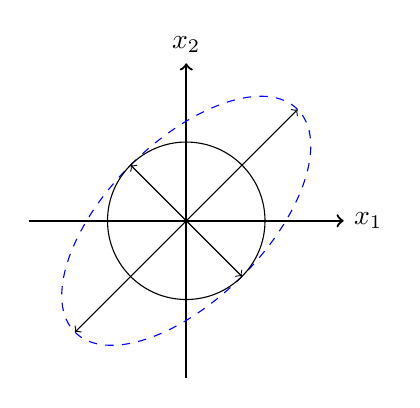
\begin{tikzpicture}
		\draw[->,thick] (-2,0) -- (2,0) node[right] {$x_1$};
		\draw[->,thick] (0,-2) -- (0,2) node[above] {$x_2$};
		\draw[->, thin] (0,0) -- (1.414,1.414);
		\draw[->, thin] (0,0) -- (-1.414,-1.414);
		\draw[->, thin] (0,0) -- (-0.707,0.707);
		\draw[->, thin] (0,0) -- (0.707,-0.707);
		\draw[dashed, rotate=+45, blue] (0,0) ellipse (2cm and 1cm);
		\draw (0,0) circle (1);
		\end{tikzpicture}
	\end{center}
\end{example}

\begin{definition}[Eigenwert, Eigenvektor, Eigenraum]
	Sind $0\neq x\in V$ und $\lambda\in K$ mit $f(x)=\lambda x$ so nennt man $\lambda$ einen \begriff{Eigenwert} von $f$ und $x$ einen \begriff{Eigenvektor} von $f$ zum Eigenwert $\lambda$. Der \begriff{Eigenraum} zu $\lambda\in K$ ist $\Eig (f,\lambda)=\{x\in V\mid f(x)=\lambda x\}$.
\end{definition}

\begin{remark}
	Für jedes $\lambda\in K$ ist $\Eig (f,\lambda)$ ein UVR von $V$, da
	\begin{align}
		\Eig (f,\lambda) &= \{x\in V\mid f(x)=\lambda x\} \notag \\
		&= \{x\in V\mid f(x)-\lambda\cdot\id_V(x)=0\} \notag \\
		&= \{x\in V\mid (f-\lambda\cdot\id_V)(x)=0\} \notag \\
		&= \Ker (f-\lambda\cdot\id_V) \notag
	\end{align}
	und $f-\lambda\cdot\id_V\in\End_K(V)$.
\end{remark}

\begin{remark}
	Achtung! Der Nullvektor ist nach Definition kein Eigenvektor, aber $\lambda=0$ kann ein Eigenwert sein, nämlich genau dann, wenn $f\notin\Aut_K(V)$, siehe Übung. Die Menge der Eigenvektoren zu $\lambda$ ist also $\Eig (f,\lambda)\backslash\{0\}$ und $\lambda$ ist genau dann ein Eigenwert von $f$, wenn $\Eig (f,\lambda)\neq\{0\}$.
\end{remark}

\begin{example}
	Ist $A=\diag(\lambda_1,...,\lambda_n)$ und $f=f_A\in\End_K(K^n)$, so sind $\lambda_1,...,\lambda_n$ EW von $f$ und jedes $e_i$ ist ein EV zum EW $\lambda_i$.
\end{example}

\begin{proposition}
	\proplbl{satz_diagonal_ev}
	Sei $B$ eine Basis von $V$. Genau dann ist $M_B(f)$ eine Diagonalmatrix, wenn $B$ aus EV von $f$ besteht.
\end{proposition}
\begin{proof}
	Ist $B=(x_1,...x_n)$ eine Basis aus EV zu EW $\lambda_1,....,\lambda_n$, so ist $M_B(f)= \diag(\lambda_1,...,\lambda_n)$ und umgekehrt.
\end{proof}

\begin{example}
	Sei $K=\real$, $V=\real^2$ und $f_{\alpha}\in\End_K(\real^2)$ die Drehung um den Winkel $\alpha\in [0,2\pi)$ \\
	\[\Rightarrow M_{\mathcal{E}}(f_{\alpha})=\begin{pmatrix}\cos(\alpha)&-\sin(\alpha) \\ \sin(\alpha) & \cos(\alpha)\end{pmatrix}\]
	Für $\alpha=0$ hat $f_{\alpha}=\id_{\real^2}$ nur den EW 1. \\
	Für $\alpha=\pi$ hat $f_{\alpha}=-\id_{\real^2}$ nur den EW -1. \\
	Für $\alpha\neq 0,\pi$ hat $f_{\alpha}$ keine EW. %TODO figure
\end{example}

\begin{lemma}
	\proplbl{lemma_EW_lin_unabh}
	Sind $\lambda_1,...,\lambda_n$ paarweise verschiedene EW von $f$ und ist $x_i$ ein EV zu $\lambda_i$ für $i=1,...,m$, so ist $(x_1,...,x_m)$ linear unabhängig.
\end{lemma}
\begin{proof}
	Induktion nach $m$\\
	\emph{$m=1$}: klar, denn $x_1\neq 0$ \\
	\emph{$m-1\to m$}: Sei $\sum_{i=1}^m \mu_i x_i=0$ mit $\mu_1,...,\mu_m\in K$.
	\begin{align}
		0&= (f-\lambda\cdot\id_V)\left( \sum\limits_{i=1}^m \mu_i x_i\right) \notag \\
		&= \sum\limits_{i=1}^m \mu_i(f(x_i)-\lambda_m\cdot x_i) \notag \\
		&= \sum\limits_{i=1}^{m-1} \mu_i(\lambda_i-\lambda_m)\cdot x_i \notag
	\end{align} 
	Nach IB ist $\mu_i(\lambda_i-\lambda_m)=0$ für $i=1,...,m-1$, da $\lambda_i\neq\lambda_m$ für $i\neq m$ also $\mu_i=0$ für $i=1,...,m-1$. Damit ist auch $\mu_m=0$. Folglich ist $(x_1,...,x_m)$ linear unabhängig.
\end{proof}

\begin{proposition}
	\proplbl{satz_eig_direkte_summe}
	Sind $\lambda_1,...,\lambda_m\in K$ paarweise verschieden, so ist 
	\[\sum\limits_{i=1}^m \Eig(f,\lambda_i)=\bigoplus_{i=0}^{m}\Eig(f,\lambda_i).\]
\end{proposition}
\begin{proof}
	Seien $x_i,y_i\in\Eig(f,\lambda_i)$ für $i=1,...,m$. Ist $\sum_{i=1}^m x_i=\sum_{i=1}^m y_i$, so ist $\sum_{i=1}^m \underbrace{x_i-y_i}_{z_i}=0$.\\
	o. E. seien $z_i\neq 0$ für $i=1,...,r$ und $z_i=0$ für $i=r+1,...,m$. Wäre $r>0$, so wären $(z_1,...,z_r)$ linear abhängig, aber $z_i=x_i-y_i\in\Eig(f,\lambda_i)\backslash\{0\}$, im Widerspruch zu \propref{lemma_EW_lin_unabh}. Somit ist $x_i=y_i$ für alle $i$ und folglich ist die Summe $\sum\Eig(f,\lambda_i)$ direkt.
\end{proof}

\begin{definition}[EW und EV für Matrizen]
	Sei $A\in\Mat_n(K)$. Man definiert Eigenwerte, Eigenvektoren, etc von $A$ als Eigenwerte, Eigenvektoren von $f_A\in\End_K(K^n)$.
\end{definition}

\begin{proposition}
	Sei $B$ eine Basis von $V$ und $\lambda\in K$. Genau dann ist $\lambda$ ein EW von $f$, wenn $\lambda$ ein EW von $A=M_B(f)$ ist. Insbesondere haben ähnliche Matrizen die selben EW.
\end{proposition}
\begin{proof}
	Dies folgt aus dem kommutativen Diagramm
	\begin{center}\begin{tikzpicture}
		\matrix (m) [matrix of math nodes,row sep=3em,column sep=4em,minimum width=2em]
		{K^n & K^n \\ V & V \\};
		\path[-stealth]
		(m-1-1) edge node [left] {$\Phi_B$} (m-2-1)
		edge node [above] {$f_A$} (m-1-2)
		(m-2-1) edge node [below] {$f$} (m-2-2)
		(m-1-2) edge node [right] {$\Phi_B$} (m-2-2);
		\end{tikzpicture}\end{center}
	denn $f_A(x)=\lambda x\iff (\Phi_B\circ f_A)(x)=\Phi_B(\lambda x)\iff f(\Phi_B(x))=\lambda\Phi_B(x)$. \\
	Ähnliche Matrizen beschreiben den selben Endomorphismus bezüglich verschiedener Basen, vgl. IV.4.1 %TODO: Verlinkung ins alte Semester
\end{proof}